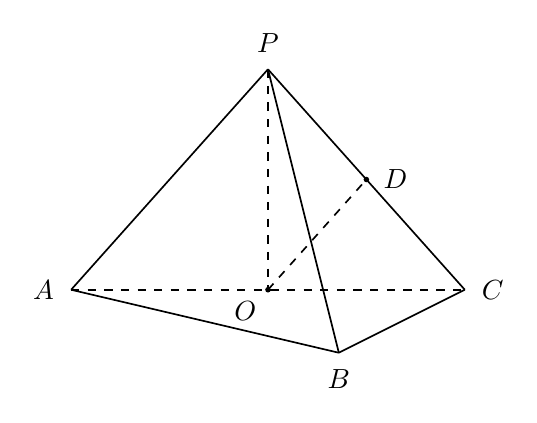
\begin{tikzpicture}[x=1cm,y=1cm,font=\normalsize,
  geometry edge/.style={solid,line width=.6pt},
  geometry label/.style={font=\normalsize,inner sep=2pt}]
% P-ABC pyramid, O midpoint of AC, D midpoint of PC (schematic projection)
\coordinate (P) at (1.5,3.2);
\coordinate (A) at (-1.0,0.4);
\coordinate (C) at (4.0,0.4);
\coordinate (B) at (2.4,-0.4);
\coordinate (O) at (1.5,0.4);
\coordinate (D) at (2.75,1.8);
% base: AB, BC solid; AC dashed (hidden)
\draw[geometry edge] (A)--(B);
\draw[geometry edge] (B)--(C);
\draw[geometry edge,dashed] (A)--(O)--(C);
% lateral
\draw[geometry edge] (P)--(A);
\draw[geometry edge] (P)--(B);
\draw[geometry edge] (P)--(C);
% interior
\draw[geometry edge,dashed] (P)--(O);
\draw[geometry edge,dashed] (O)--(D);
\fill (O) circle (1pt);
\fill (D) circle (1pt);
% labels offset from strokes
\node[geometry label,above=4pt] at (P) {$P$};
\node[geometry label,left=4pt] at (A) {$A$};
\node[geometry label,right=4pt] at (C) {$C$};
\node[geometry label,below=4pt] at (B) {$B$};
\node[geometry label,below left=2pt] at (O) {$O$};
\node[geometry label,right=4pt] at (D) {$D$};
\end{tikzpicture}
